\section{Prototipação de Baixa Fidelidade}

\subsection{Cenário Textual}

Ao não se sentir bem, um usuário busca na internet por um sistema de diagnóstico online.
Esse usuário sabe que simplesmente buscar por sintomas de maneira isolada não leva a dados concretos.

Nesse contexto, este usuário encontra o sistema HealthWeb, onde, após concordar com os termos de uso, preenche alguns dados simples, como sexo, idade e peso, então segue para um questionário com perguntas do tipo sim e não a respeito de sintomas que tem ou teve desde que começou a se sentir mal.

Em seguida, uma lista de possíveis diagnósticos baseados nos sintomas, ordenados por probabilidade, começando pelo mais provável. Cada item da lista pode ser selecionado, apresentando uma pequena página com informações a respeito dessa doença, com a possibilidade de acessar a página completa a respeito desta doença.

\subsection{Proposta de logomarca}

A logomarca proposta, apresentada na figura \ref{fig:logomarca}, consiste no título ``HealthWeb'' tipografado em fonte ``Cinzel Decorative''.

\begin{figure}[hbtp]
	\centering
	
\includegraphics[width=\textwidth]{figure/logo.png}
	\caption{Logomarca proposta.}
	\label{fig:logomarca}
\end{figure}

\subsection{Tarefas realizadas pelos sistema}

Este sistema realiza a seguinte lista de tarefas:
\begin{itemize}
	\item Transitar entre páginas de informações sobre o sistema;
	\item Listar e detalhar doenças cadastradas no banco de dados;
	\item Coletar informações do usuário que serão utilizadas para o diagnóstico;
	\item Listar possíveis doenças, apresentando parâmetro estatístico, correlacionando os sintomas denotados com o banco de dados sobre doenças;
\end{itemize}

\subsection{Storyboard}

\subsubsection{Versão mobile}

\begin{figure}[htbp]
	\centering
	\hspace{0.24\linewidth}
	\hfill
	\begin{subfigure}{0.24\linewidth}
		\centering
		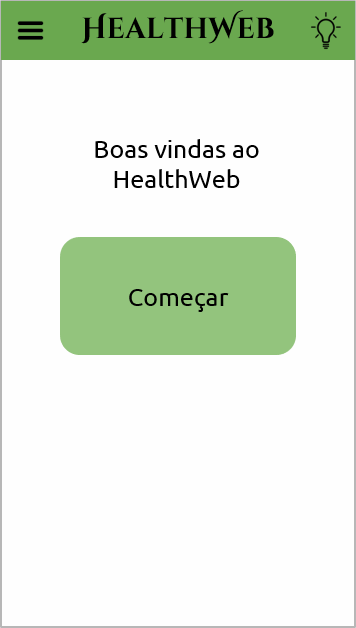
\includegraphics[width=\linewidth]{figure/prototype/mobile/home.png}
		\caption{Tela de início.}
		\label{fig:mobile:home}
	\end{subfigure}
\hfill
	\begin{subfigure}{0.24\linewidth}
		\centering
		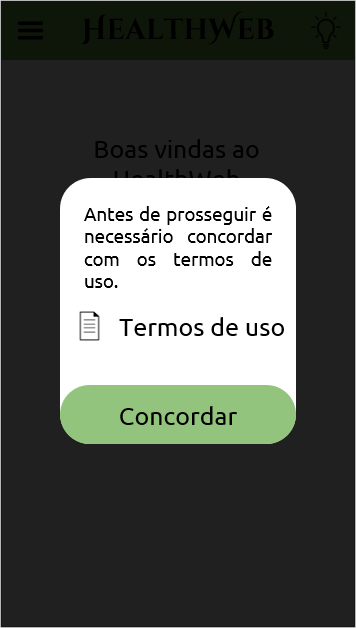
\includegraphics[width=\linewidth]{figure/prototype/mobile/agreeing.png}
		\caption{Concordar com termos.}
		\label{fig:mobile:agreeing}
	\end{subfigure}
\hfill
\hspace{0.24\linewidth}
	\caption{Interface Inicial.}
	\label{fig:mobile:home_agreeing}
\end{figure}

\begin{figure}[htbp]
	\centering
	\begin{subfigure}{0.24\linewidth}
		\centering
		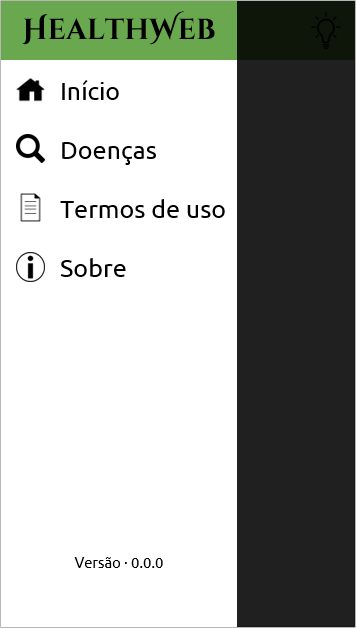
\includegraphics[width=\linewidth]{figure/prototype/mobile/drawer.png}
		\caption{Menu lateral.}
		\label{fig:mobile:drawer}
	\end{subfigure}
	\hfill
	\begin{subfigure}{0.24\linewidth}
		\centering
		
\includegraphics[width=\linewidth]{figure/prototype/mobile/about.png}
		\caption{Tela sobre.}
		\label{fig:mobile:about}
	\end{subfigure}
	\hfill
	\begin{subfigure}{0.24\linewidth}
		\centering
		
\includegraphics[width=\linewidth]{figure/prototype/mobile/terms.png}
		\caption{Tela de termos de uso.}
		\label{fig:mobile:terms}
	\end{subfigure}
	\hfill
	\begin{subfigure}{0.24\linewidth}
		\centering
		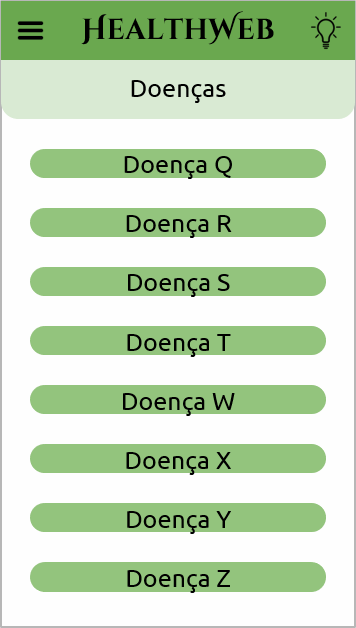
\includegraphics[width=\linewidth]{figure/prototype/mobile/list_disease.png}
		\caption{Lista de doenças.}
		\label{fig:mobile:list_disease}
	\end{subfigure}
	\caption{Menu e páginas de documentação.}
	\label{fig:mobile:drawer_about_terms_list_disease}
\end{figure}

\begin{figure}[htbp]
	\centering
	\begin{subfigure}{0.24\linewidth}
		\centering
		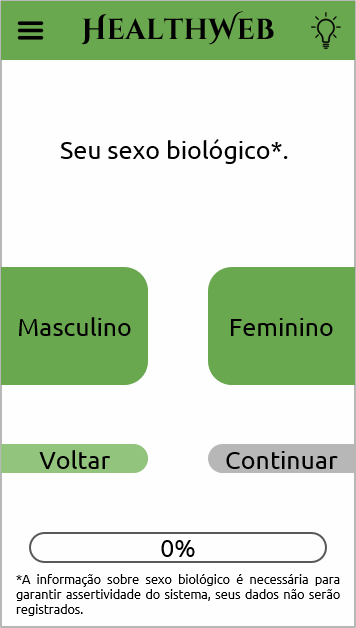
\includegraphics[width=\linewidth]{figure/prototype/mobile/bio_sex.png}
		\caption{Sexo biológico.}
		\label{fig:mobile:bio_sex}
	\end{subfigure}
	\hfill
	\begin{subfigure}{0.24\linewidth}
		\centering
		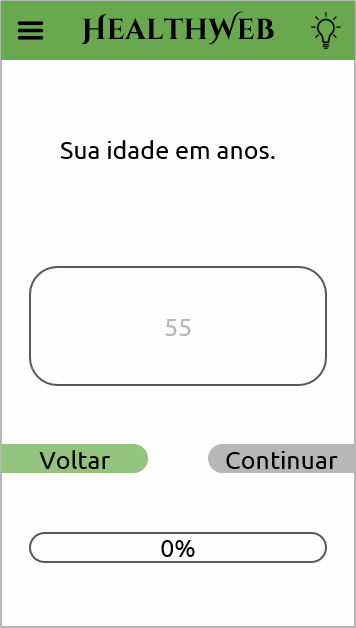
\includegraphics[width=\linewidth]{figure/prototype/mobile/age.png}
		\caption{Idade.}
		\label{fig:mobile:age}
	\end{subfigure}
	\hfill
	\begin{subfigure}{0.24\linewidth}
		\centering
		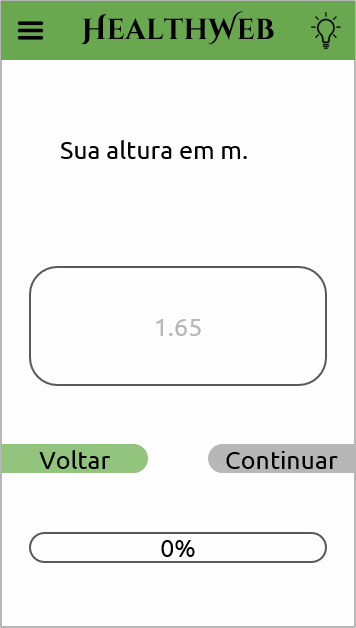
\includegraphics[width=\linewidth]{figure/prototype/mobile/height.png}
		\caption{Altura.}
		\label{fig:mobile:height}
	\end{subfigure}
	\hfill
	\begin{subfigure}{0.24\linewidth}
		\centering
		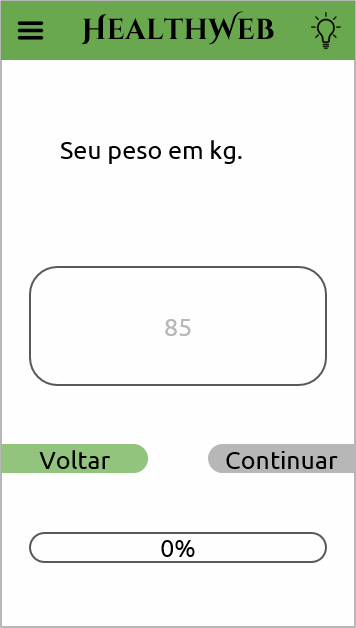
\includegraphics[width=\linewidth]{figure/prototype/mobile/weight.png}
		\caption{Peso.}
		\label{fig:mobile:weight}
	\end{subfigure}
	\caption{Perguntas sobre informações básicas do usuário.}
	\label{fig:mobile:bio_sex_age_height_weight}
\end{figure}

\begin{figure}[htbp]
	\centering
	\hspace{0.11\linewidth}
	\hfill
	\begin{subfigure}{0.24\linewidth}
		\centering
		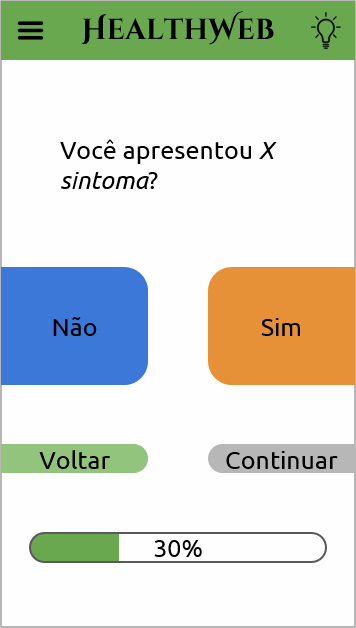
\includegraphics[width=\linewidth]{figure/prototype/mobile/symptom.png}
		\caption{Antes da resposta.}
		\label{fig:mobile:symptom}
	\end{subfigure}
	\hfill
	\begin{subfigure}{0.24\linewidth}
		\centering
		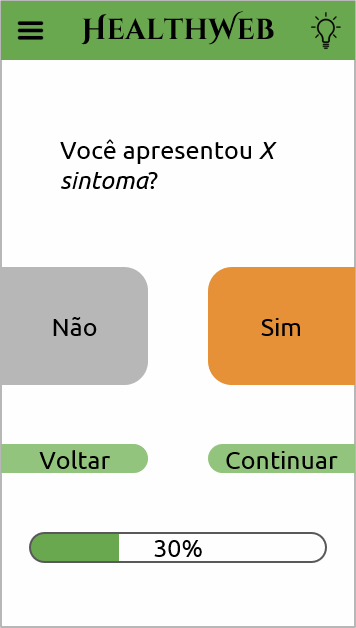
\includegraphics[width=\linewidth]{figure/prototype/mobile/symptom_yes.png}
		\caption{Resposta positiva.}
		\label{fig:mobile:symptom_yes}
	\end{subfigure}
	\hfill
	\begin{subfigure}{0.24\linewidth}
		\centering
		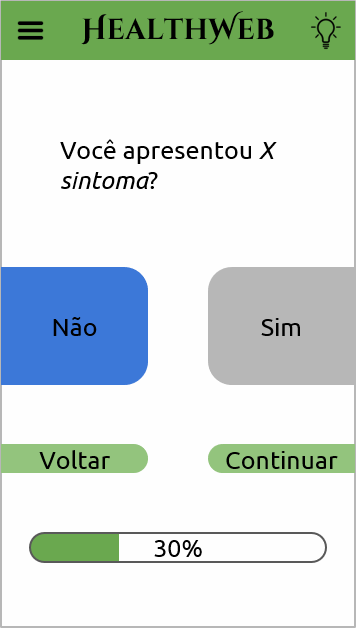
\includegraphics[width=\linewidth]{figure/prototype/mobile/symptom_no.png}
		\caption{Resposta negativa.}
		\label{fig:mobile:symptom_no}
	\end{subfigure}
	\hspace{0.11\linewidth}
	\hfill
	\caption{Interface durante questionário de sintomas.}
	\label{fig:mobile:symptom_yes_no}
\end{figure}

\begin{figure}[htbp]
	\centering
	\begin{subfigure}{0.24\linewidth}
		\centering
		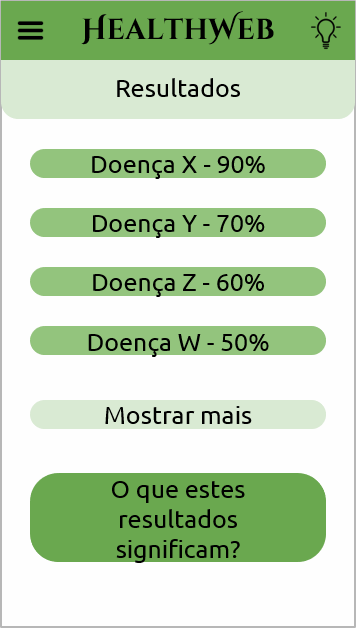
\includegraphics[width=\linewidth]{figure/prototype/mobile/results.png}
		\caption{Resultados.}
		\label{fig:mobile:results}
	\end{subfigure}
	\hfill
	\begin{subfigure}{0.24\linewidth}
		\centering
		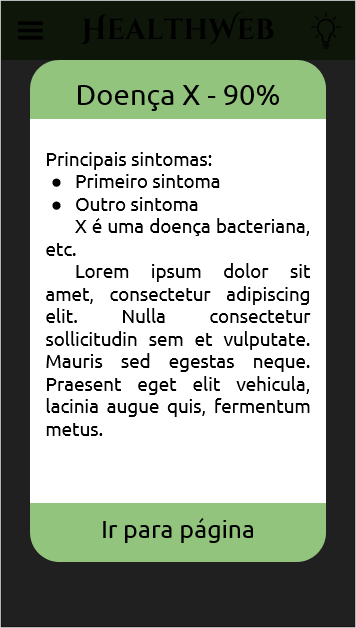
\includegraphics[width=\linewidth]{figure/prototype/mobile/this_disease.png}
		\caption{Resumo sobre doença.}
		\label{fig:mobile:this_disease}
	\end{subfigure}
	\hfill
	\begin{subfigure}{0.24\linewidth}
		\centering
		
\includegraphics[width=\linewidth]{figure/prototype/mobile/disease_page.png}
		\caption{Página sobre doença.}
		\label{fig:mobile:disease_page}
	\end{subfigure}
	\hfill
	\begin{subfigure}{0.24\linewidth}
		\centering
		
\includegraphics[width=\linewidth]{figure/prototype/mobile/meaning.png}
		\caption{Explicação.}
		\label{fig:mobile:meaning}
	\end{subfigure}
	\caption{Interface de detalhamento e resultados.}
	\label{fig:mobile:results_this_disease_disease_page_meaning}
\end{figure}

\begin{figure}[htbp]
	\centering
	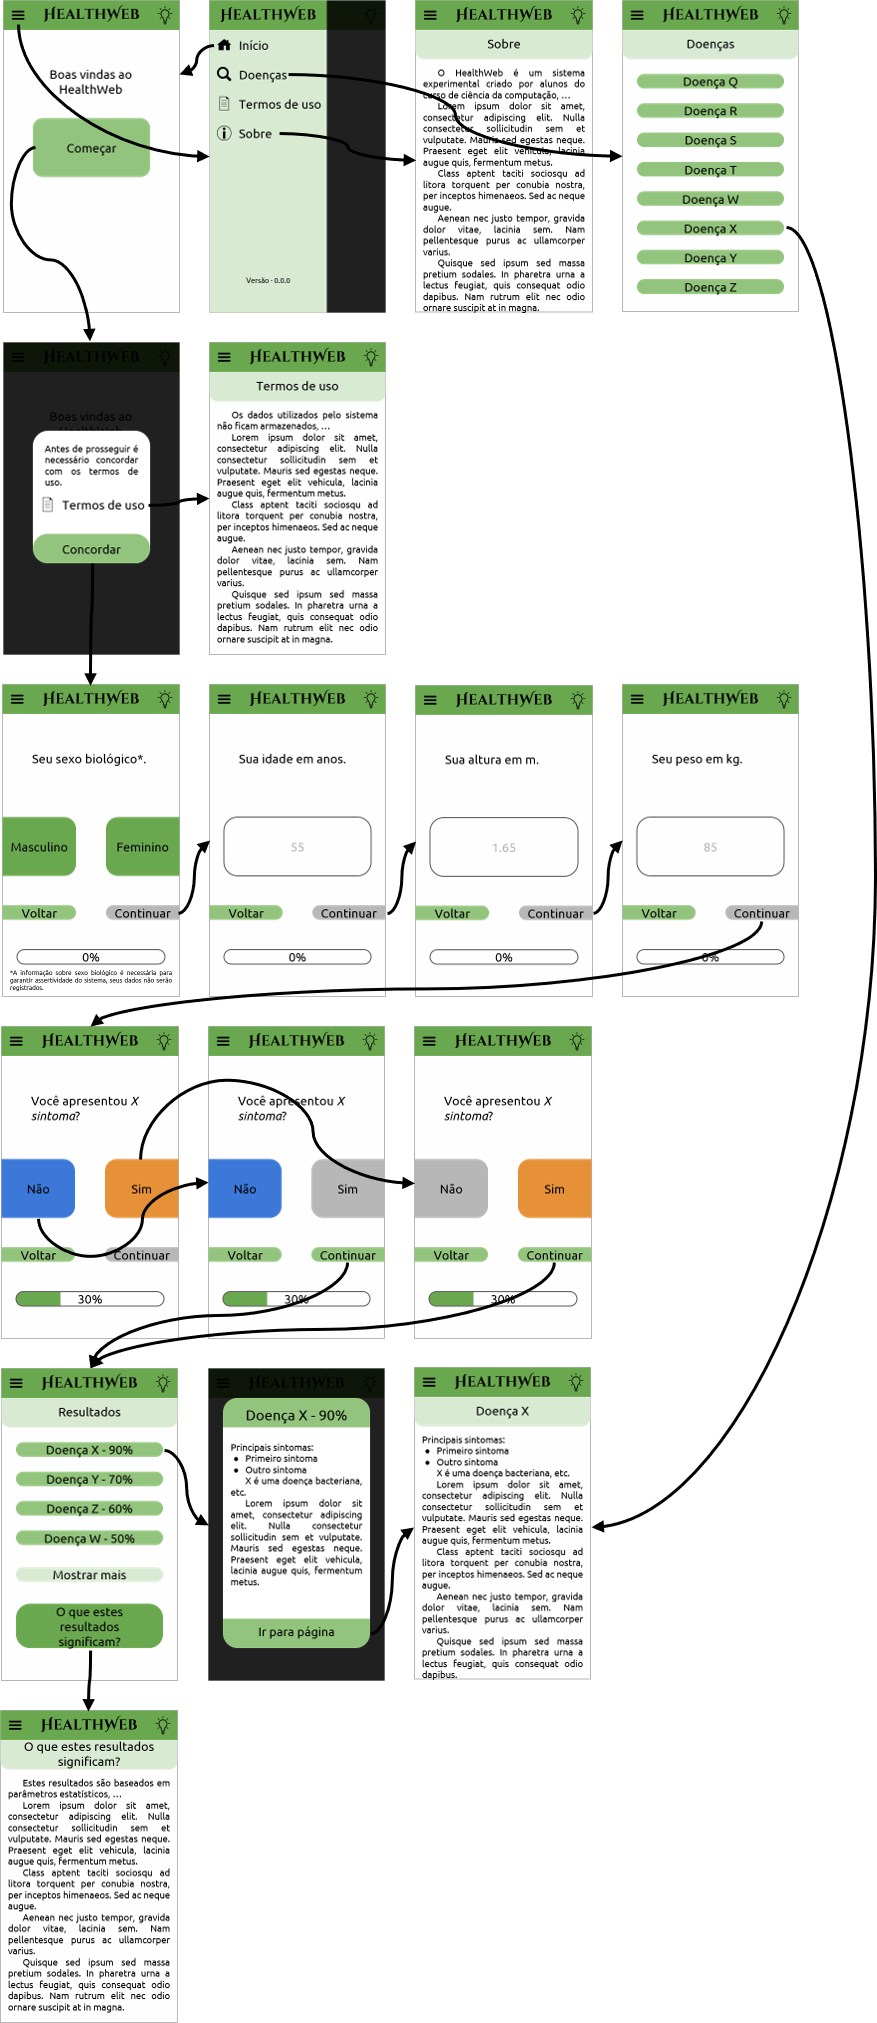
\includegraphics[width=\linewidth]{figure/prototype/mobile/storyboard.png}
	\caption{Storyboard para versão mobile.}
	\label{fig:mobile:story}
\end{figure}

\subsubsection{Versão desktop}

\begin{figure}[htbp]
	\centering
	\begin{subfigure}{0.49\linewidth}
		\centering
		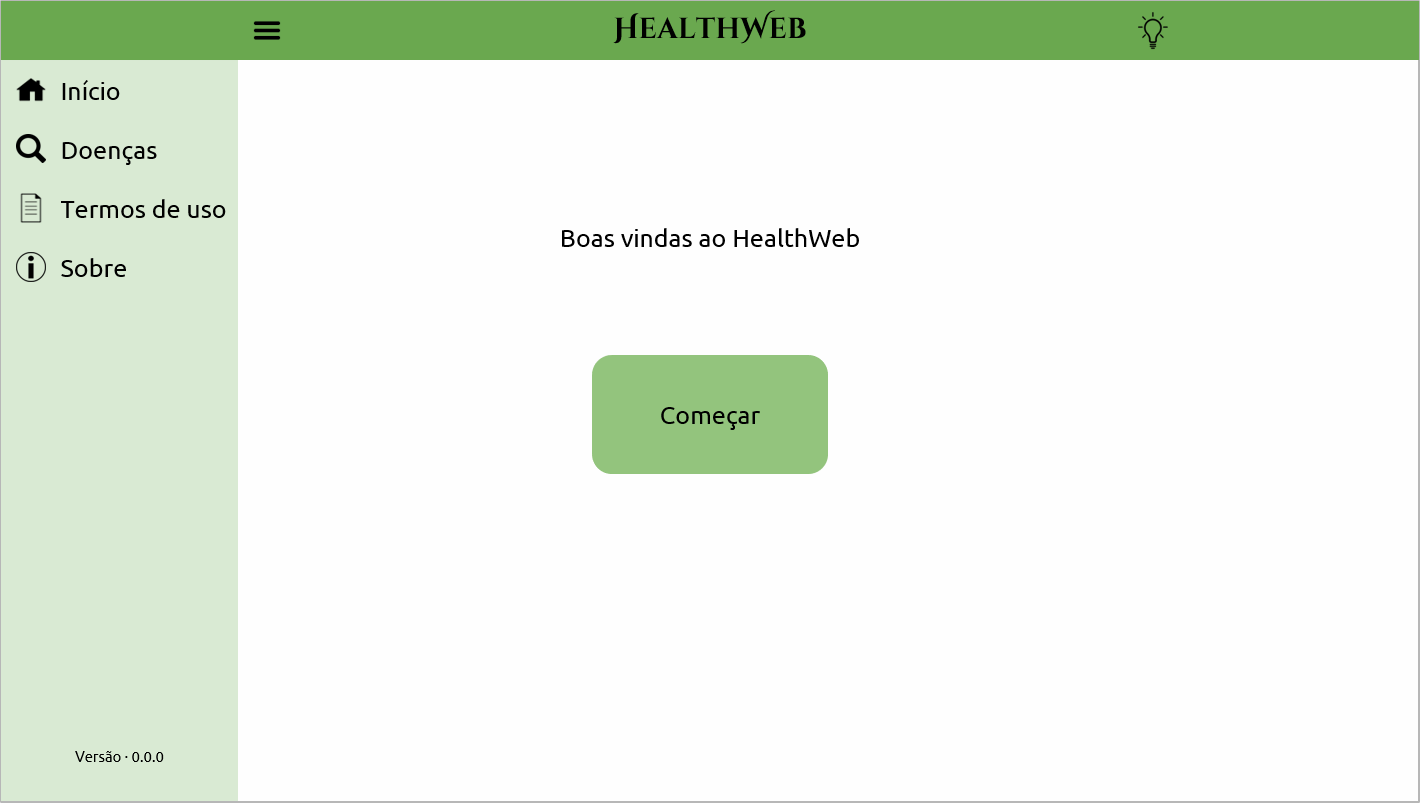
\includegraphics[width=\linewidth]{figure/prototype/desktop/home.png}
		\caption{Tela de início.}
		\label{fig:desktop:home}
	\end{subfigure}
	\hfill
	\begin{subfigure}{0.49\linewidth}
		\centering
		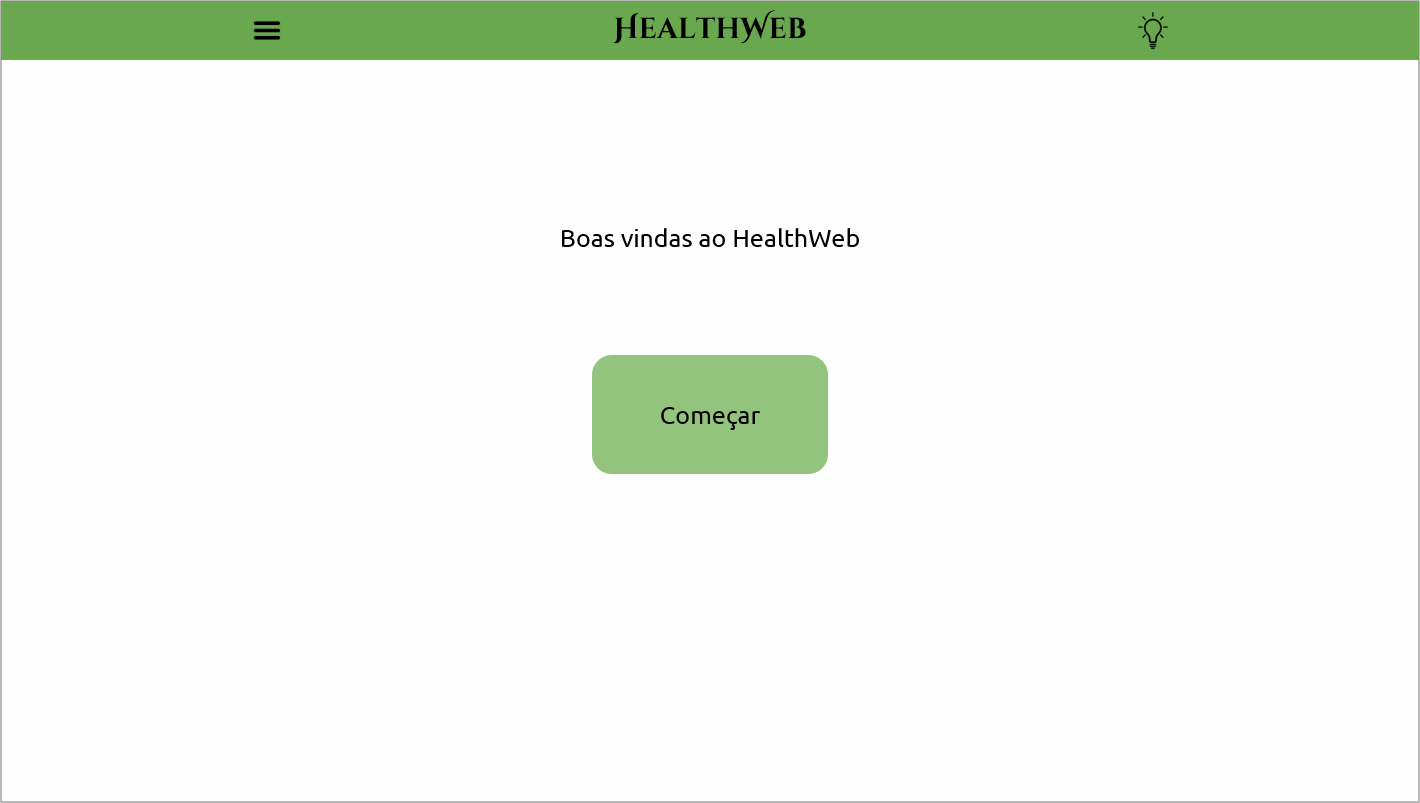
\includegraphics[width=\linewidth]{figure/prototype/desktop/drawer.png}
		\caption{Menu lateral recolhido na tela de início.}
		\label{fig:desktop:drawer}
	\end{subfigure}
	\caption{Tela de início e detalhe do menu lateral.}
	\label{fig:desktop:home_agreeing}
\end{figure}

\begin{figure}[htbp]
	\centering
	\begin{subfigure}{0.49\linewidth}
		\centering
		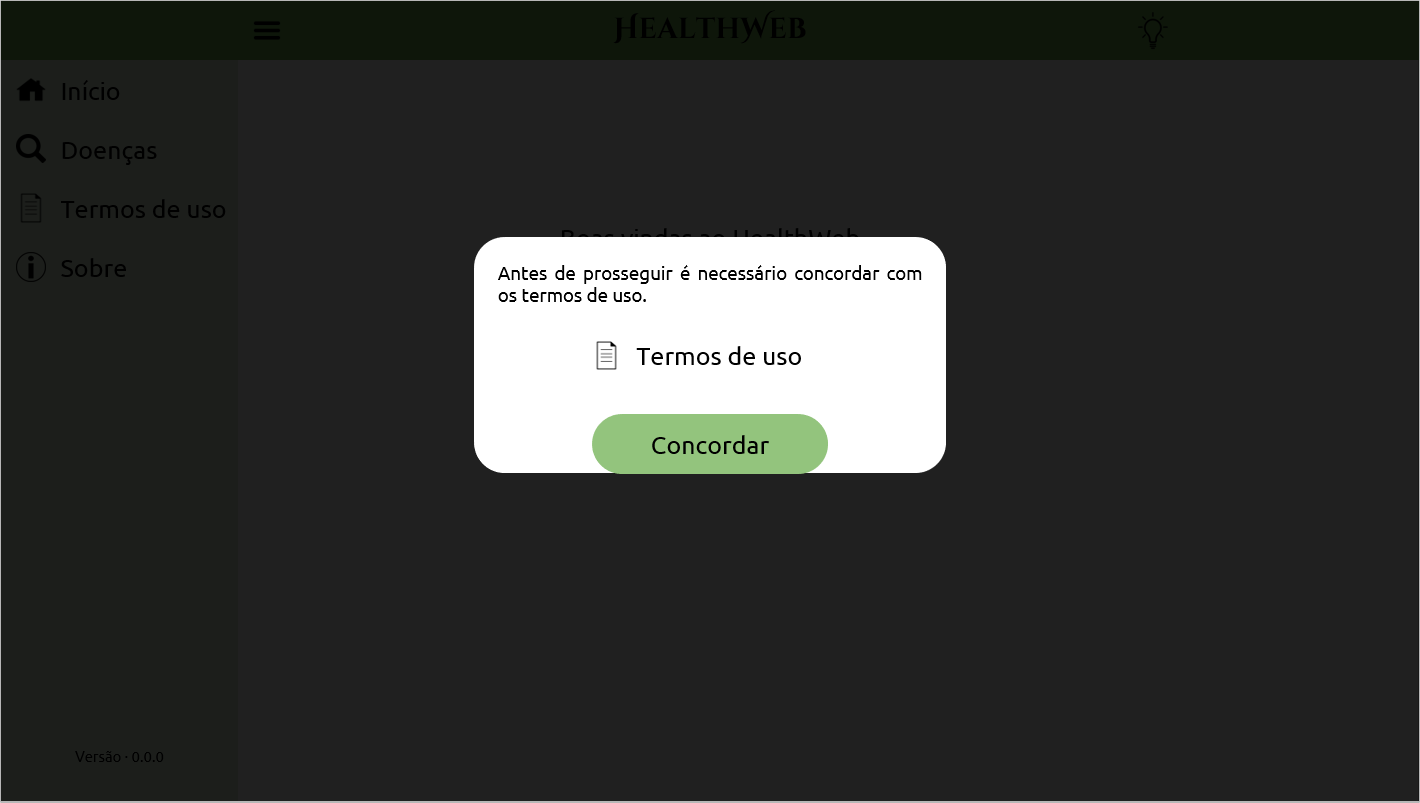
\includegraphics[width=\linewidth]{figure/prototype/desktop/agreeing.png}
		\caption{Concordar com termos.}
		\label{fig:desktop:agreeing}
	\end{subfigure}
	\hfill
	\begin{subfigure}{0.49\linewidth}
		\centering
		
\includegraphics[width=\linewidth]{figure/prototype/desktop/about.png}
		\caption{Tela sobre.}
		\label{fig:desktop:about}
	\end{subfigure}
	\hfill
	\begin{subfigure}{0.49\linewidth}
		\centering
		
\includegraphics[width=\linewidth]{figure/prototype/desktop/terms.png}
		\caption{Tela de termos de uso.}
		\label{fig:desktop:terms}
	\end{subfigure}
	\hfill
	\begin{subfigure}{0.49\linewidth}
		\centering
		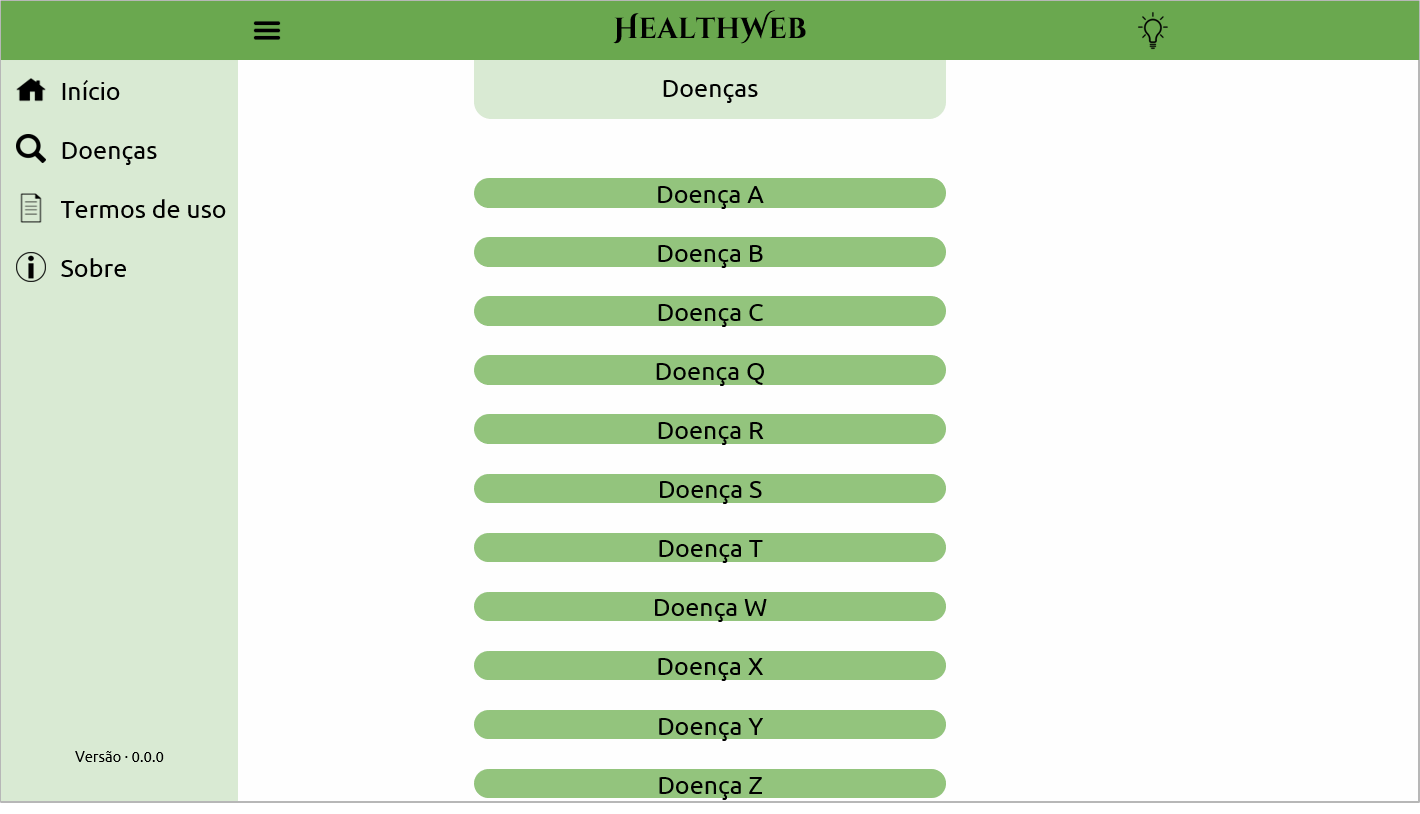
\includegraphics[width=\linewidth]{figure/prototype/desktop/list_disease.png}
		\caption{Lista de doenças.}
		\label{fig:desktop:list_disease}
	\end{subfigure}
	\caption{Páginas de documentação.}
	\label{fig:desktop:drawer_about_terms_list_disease}
\end{figure}

\begin{figure}[htbp]
	\centering
	\begin{subfigure}{0.49\linewidth}
		\centering
		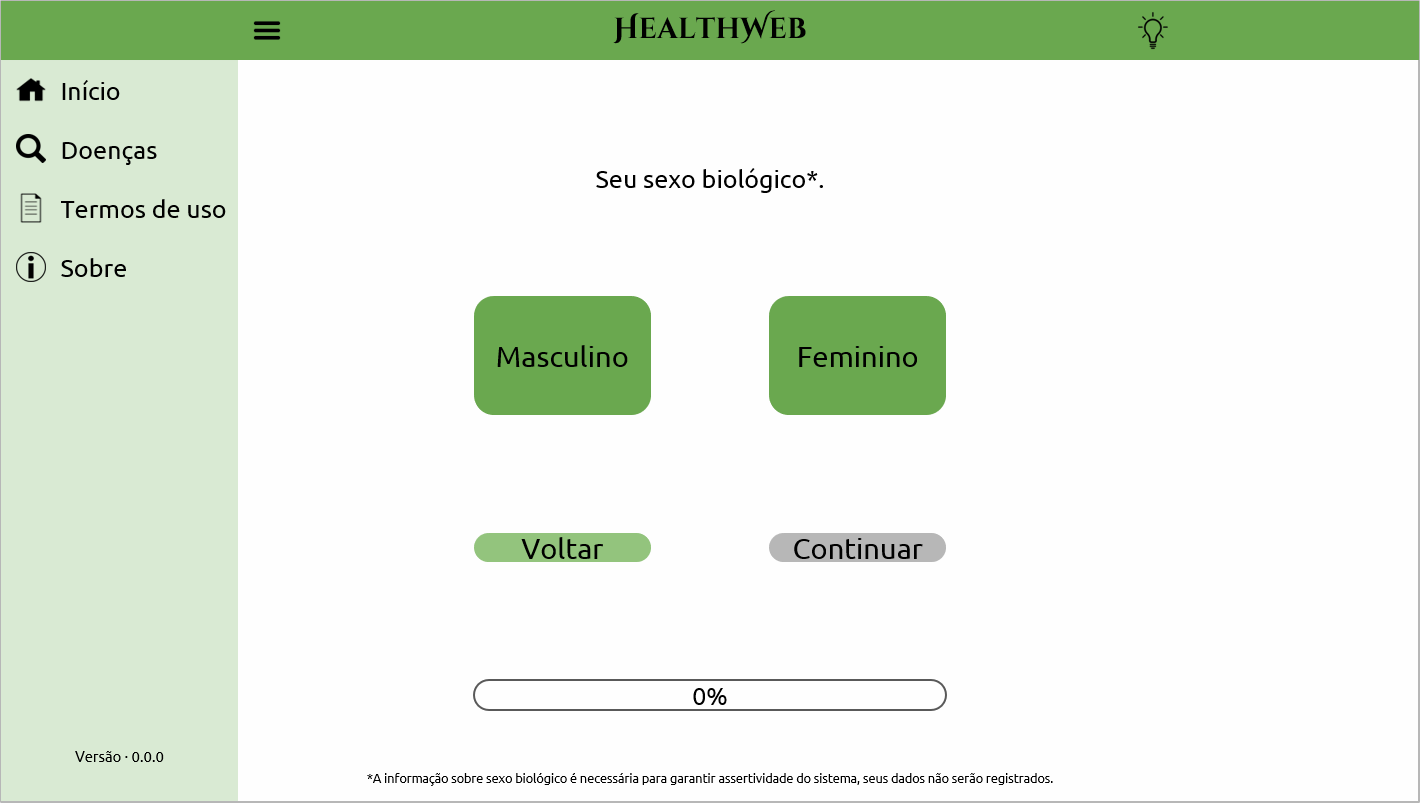
\includegraphics[width=\linewidth]{figure/prototype/desktop/bio_sex.png}
		\caption{Sexo biológico.}
		\label{fig:desktop:bio_sex}
	\end{subfigure}
	\hfill
	\begin{subfigure}{0.49\linewidth}
		\centering
		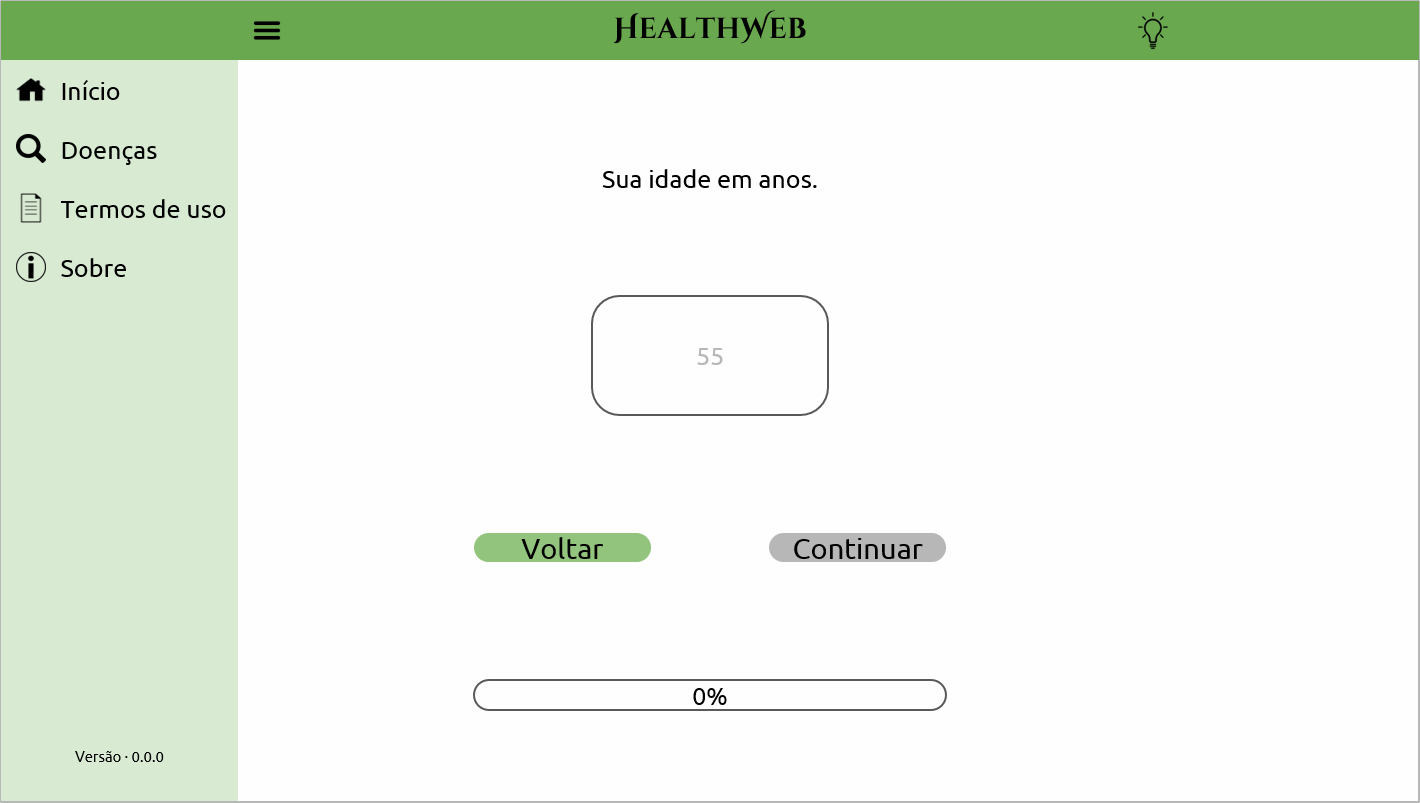
\includegraphics[width=\linewidth]{figure/prototype/desktop/age.png}
		\caption{Idade.}
		\label{fig:desktop:age}
	\end{subfigure}
	\hfill
	\begin{subfigure}{0.49\linewidth}
		\centering
		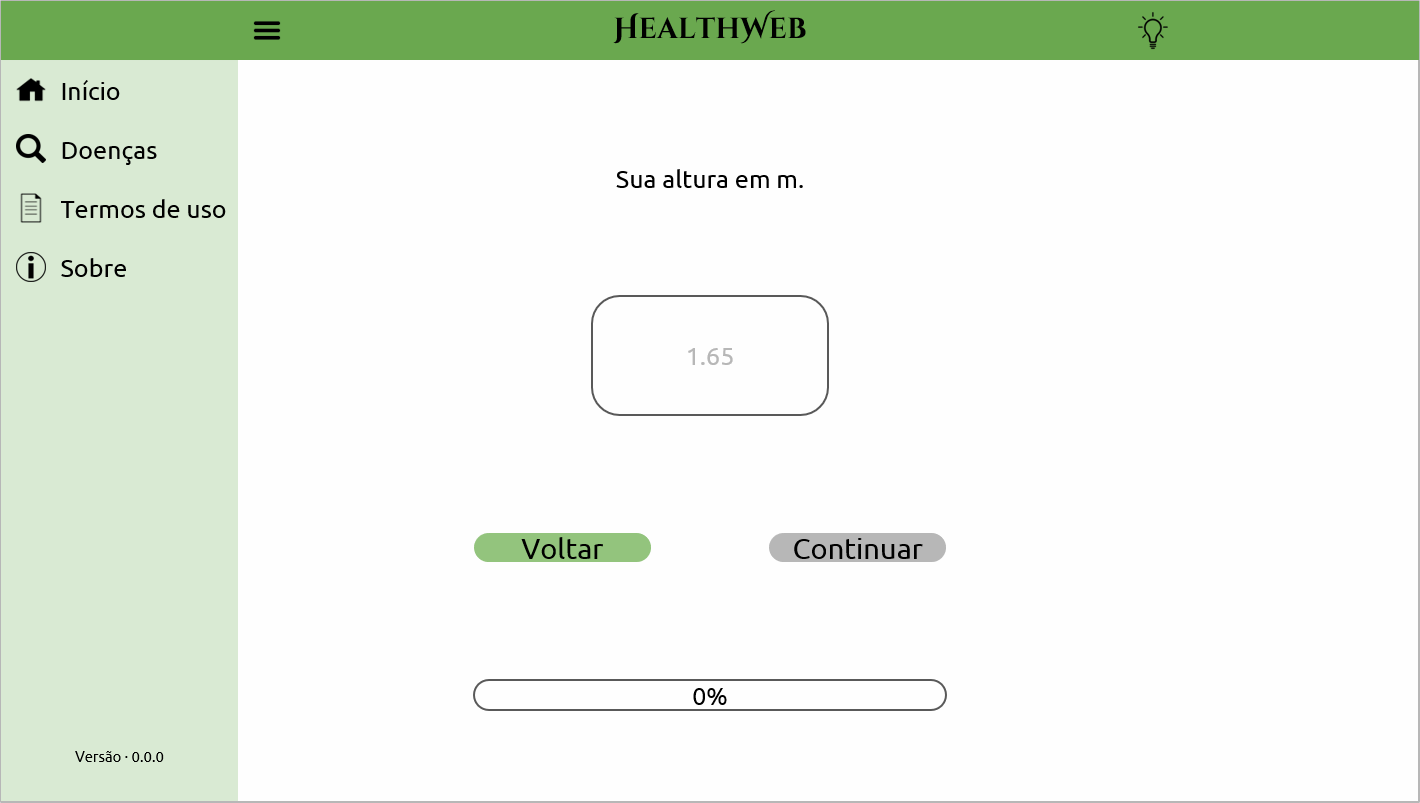
\includegraphics[width=\linewidth]{figure/prototype/desktop/height.png}
		\caption{Altura.}
		\label{fig:desktop:height}
	\end{subfigure}
	\hfill
	\begin{subfigure}{0.49\linewidth}
		\centering
		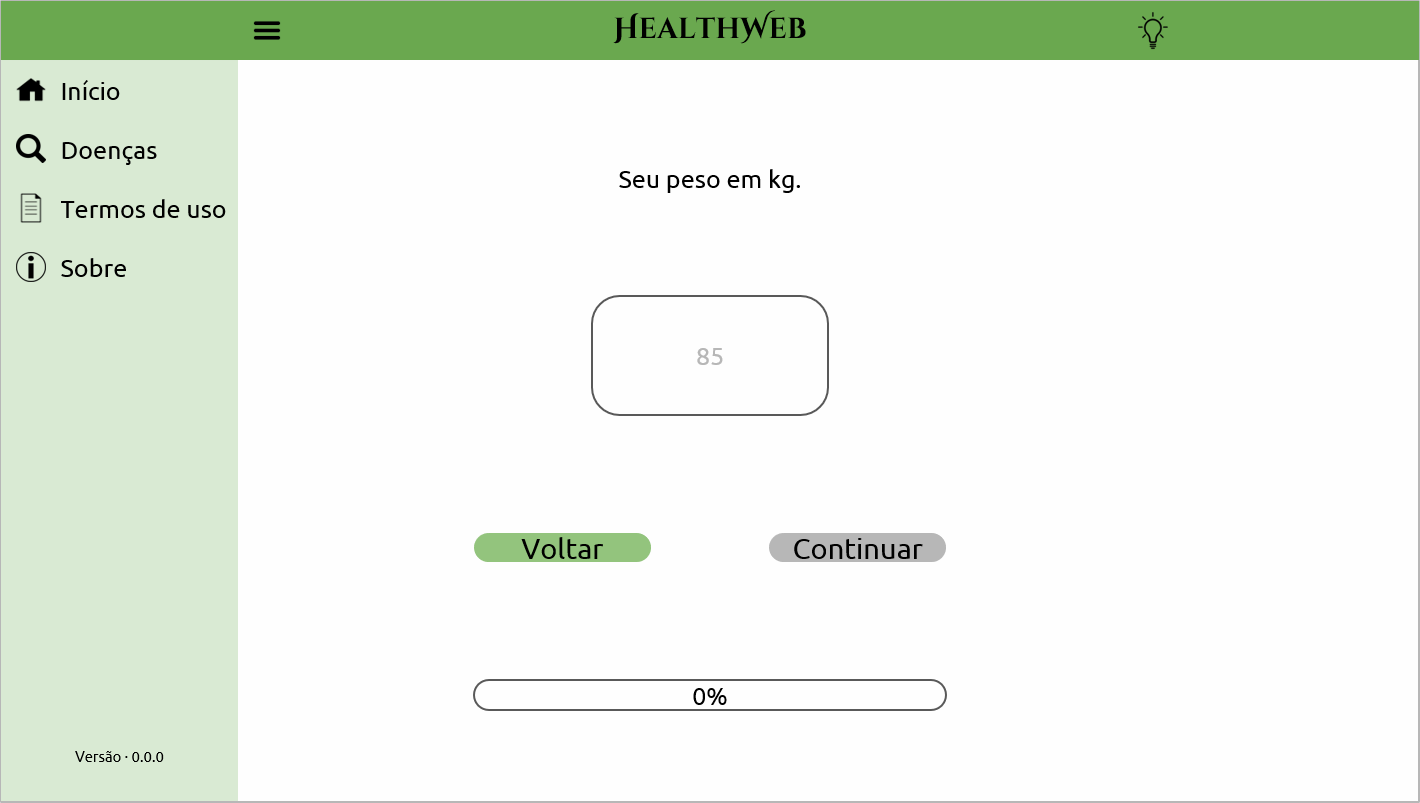
\includegraphics[width=\linewidth]{figure/prototype/desktop/weight.png}
		\caption{Peso.}
		\label{fig:desktop:weight}
	\end{subfigure}
	\caption{Perguntas sobre informações básicas do usuário.}
	\label{fig:desktop:bio_sex_age_height_weight}
\end{figure}

\begin{figure}[htbp]
	\centering
	\begin{subfigure}{0.49\linewidth}
		\centering
		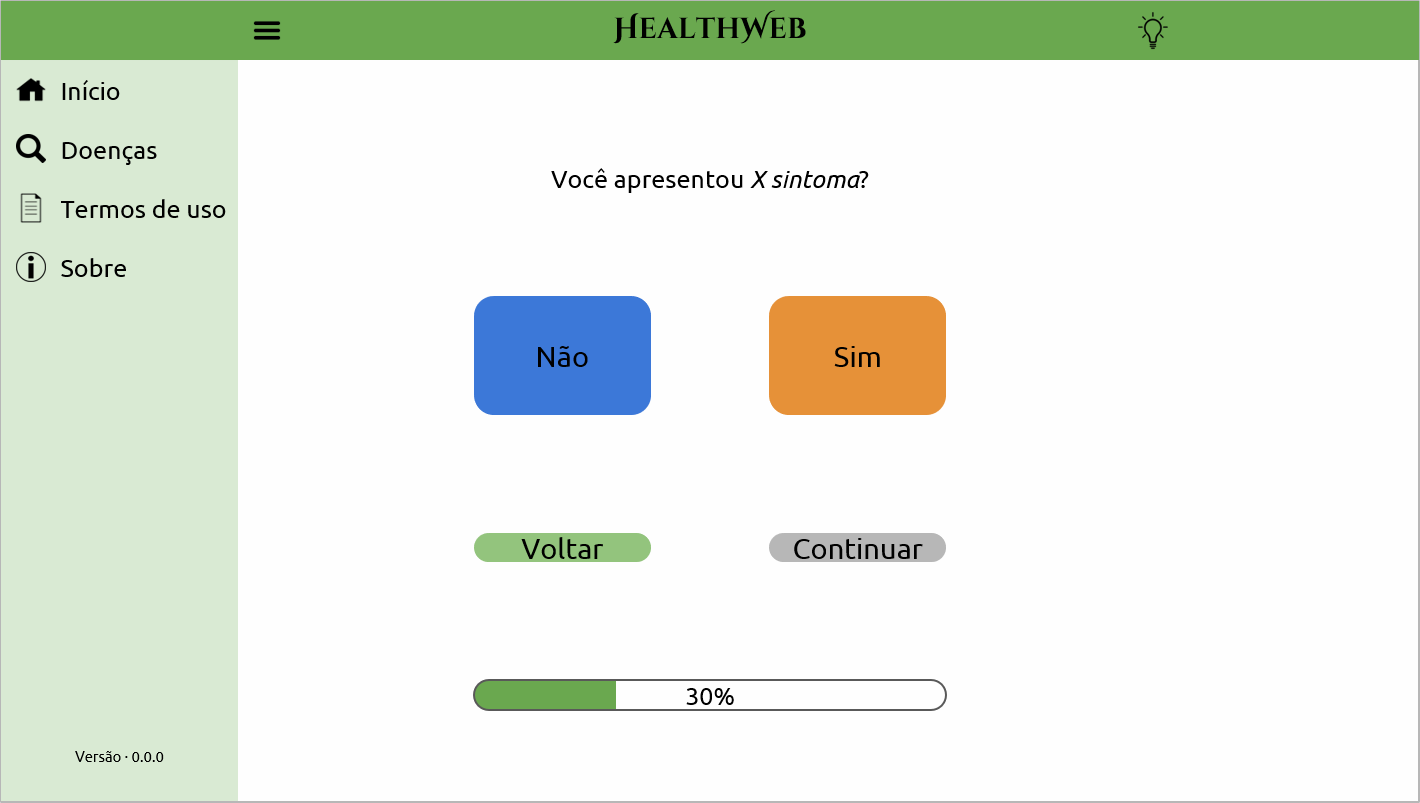
\includegraphics[width=\linewidth]{figure/prototype/desktop/symptom.png}
		\caption{Antes da resposta.}
		\label{fig:desktop:symptom}
	\end{subfigure}
	\linebreak
	\begin{subfigure}{0.49\linewidth}
		\centering
		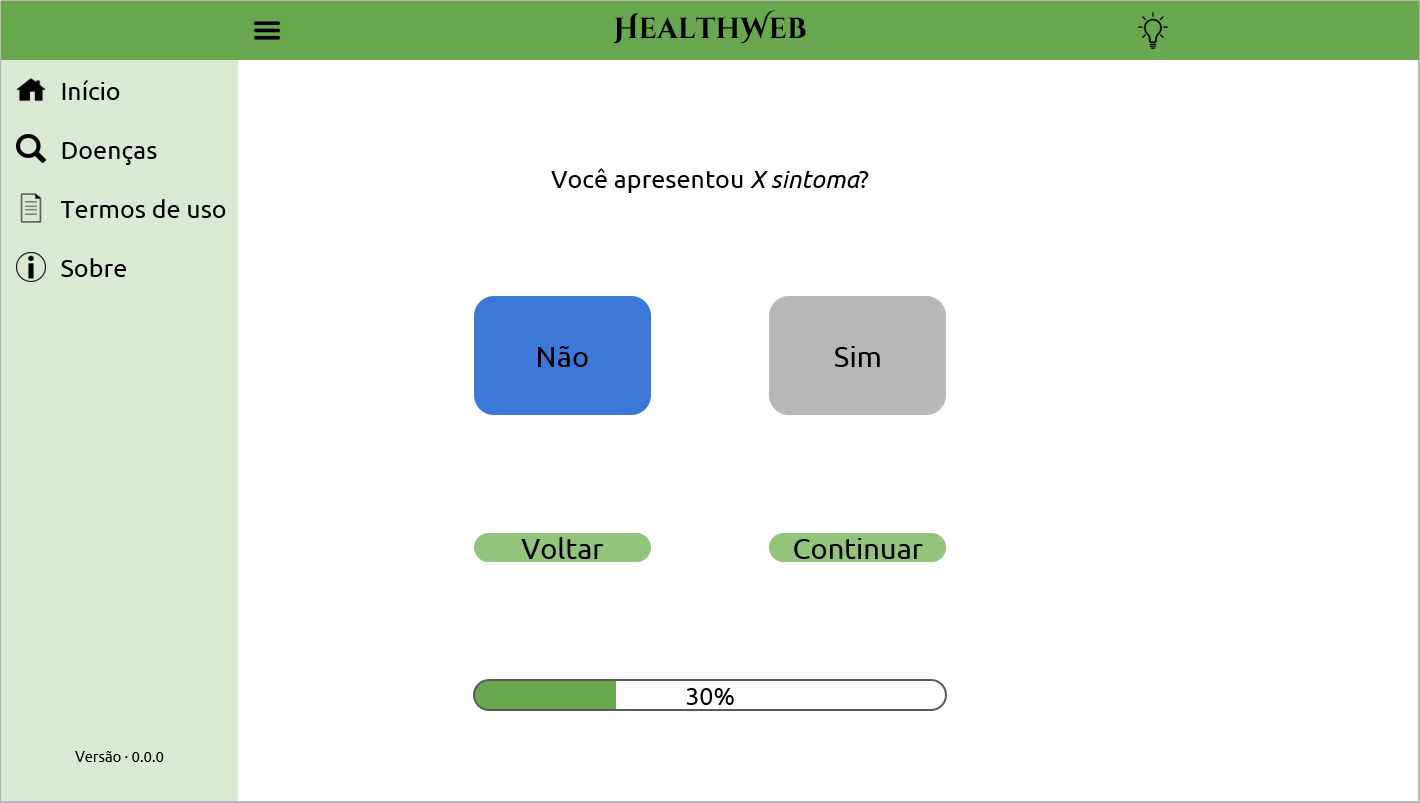
\includegraphics[width=\linewidth]{figure/prototype/desktop/symptom_no.png}
		\caption{Resposta negativa.}
		\label{fig:desktop:symptom_no}
	\end{subfigure}
	\hfill
	\begin{subfigure}{0.49\linewidth}
		\centering
		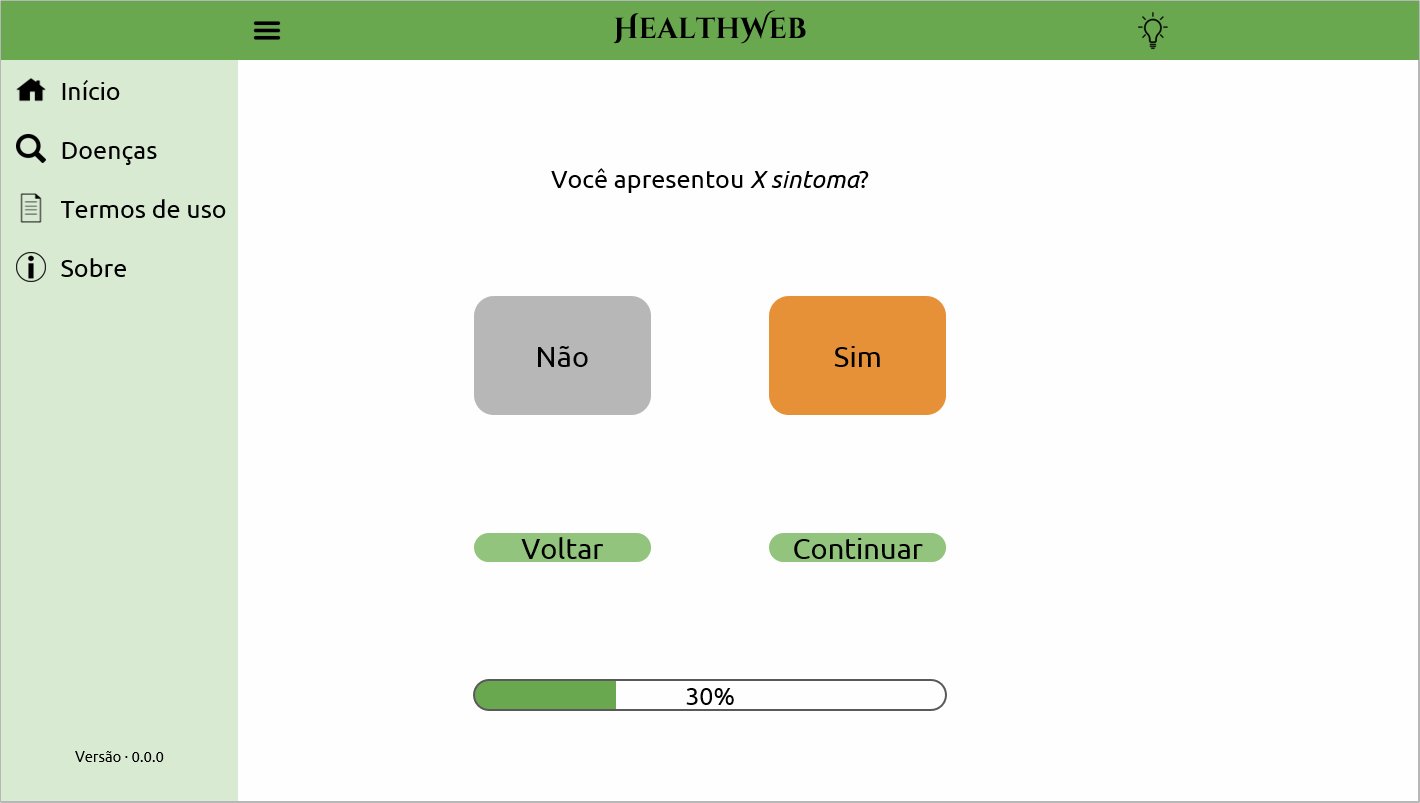
\includegraphics[width=\linewidth]{figure/prototype/desktop/symptom_yes.png}
		\caption{Resposta positiva.}
		\label{fig:desktop:symptom_yes}
	\end{subfigure}
	\hfill
	\caption{Interface durante questionário de sintomas.}
	\label{fig:desktop:symptom_yes_no}
\end{figure}

\begin{figure}[htbp]
	\centering
	\begin{subfigure}{0.49\linewidth}
		\centering
		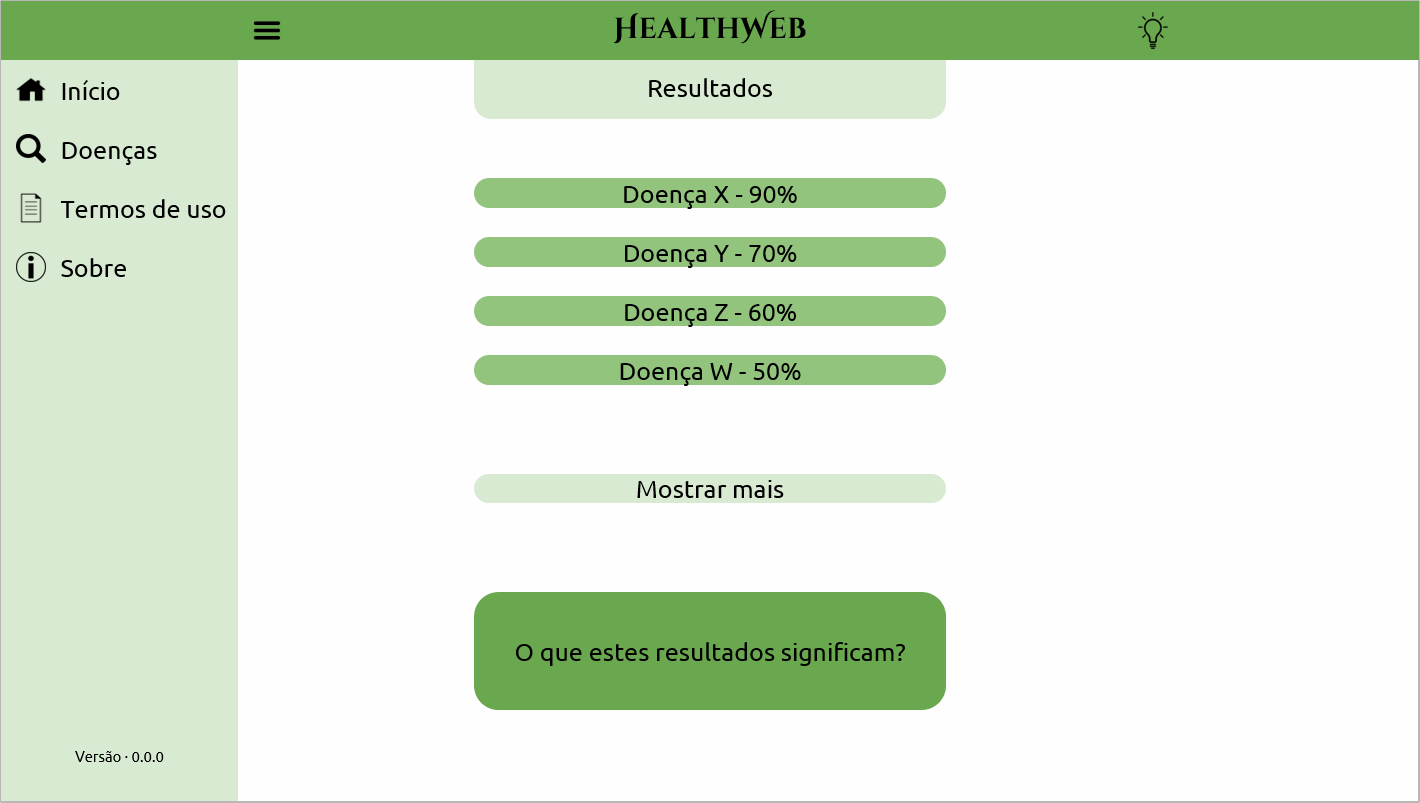
\includegraphics[width=\linewidth]{figure/prototype/desktop/results.png}
		\caption{Resultados.}
		\label{fig:desktop:results}
	\end{subfigure}
	\hfill
	\begin{subfigure}{0.49\linewidth}
		\centering
		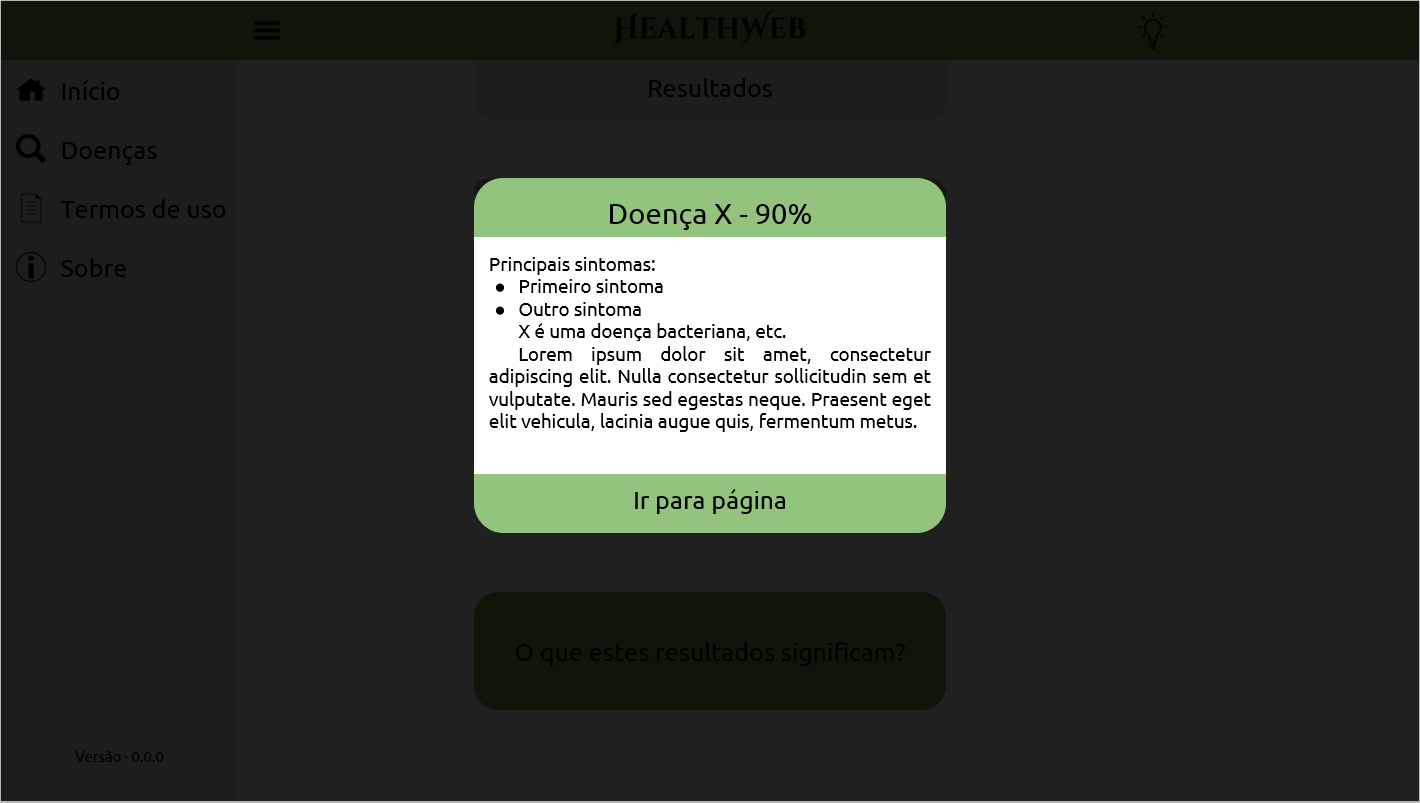
\includegraphics[width=\linewidth]{figure/prototype/desktop/this_disease.png}
		\caption{Resumo sobre doença.}
		\label{fig:desktop:this_disease}
	\end{subfigure}
	\hfill
	\begin{subfigure}{0.49\linewidth}
		\centering
		
\includegraphics[width=\linewidth]{figure/prototype/desktop/disease_page.png}
		\caption{Página sobre doença.}
		\label{fig:desktop:disease_page}
	\end{subfigure}
	\hfill
	\begin{subfigure}{0.49\linewidth}
		\centering
		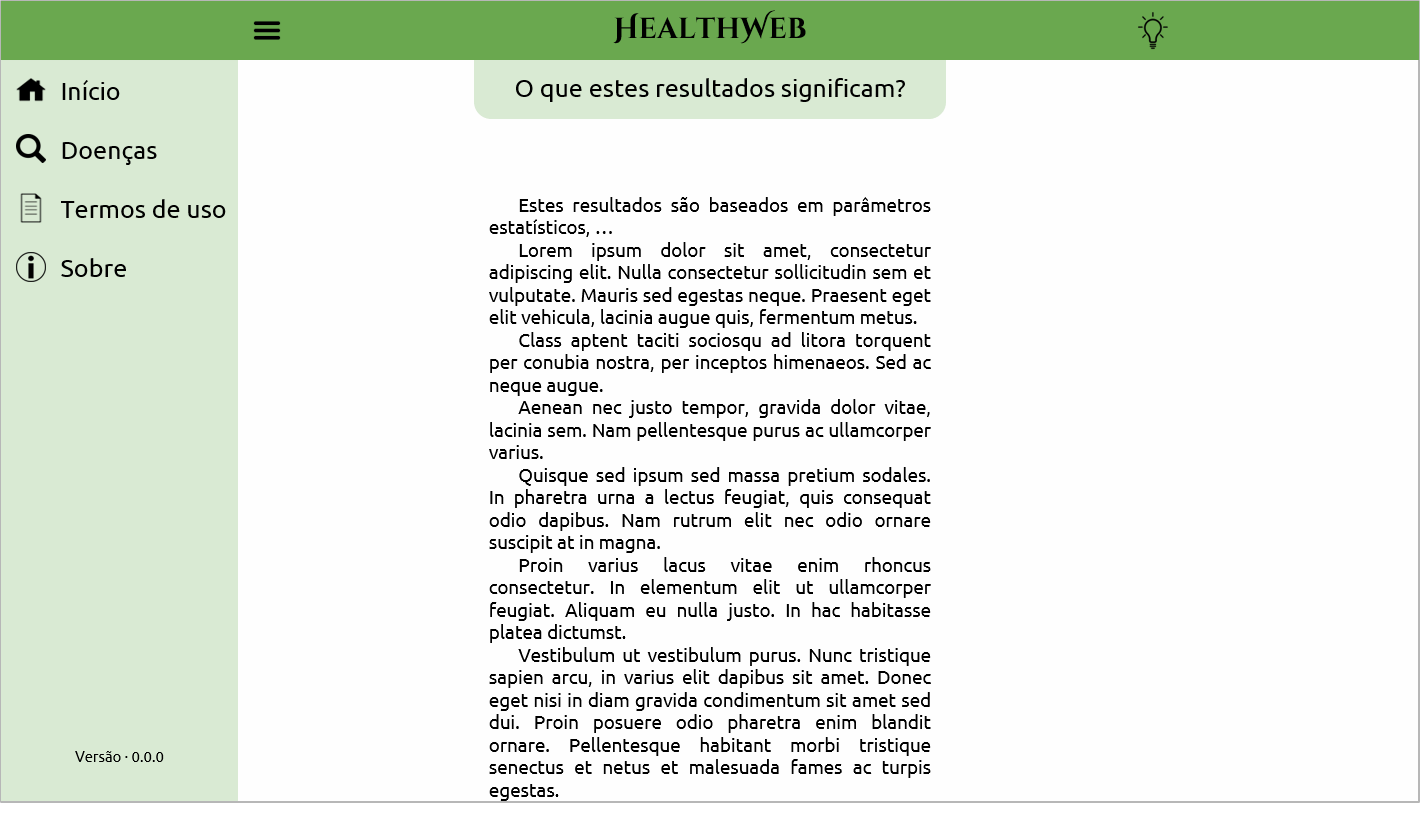
\includegraphics[width=\linewidth]{figure/prototype/desktop/meaning.png}
		\caption{Explicação.}
		\label{fig:desktop:meaning}
	\end{subfigure}
	\caption{Interface de detalhamento e resultados.}
	\label{fig:desktop:results_this_disease_disease_page_meaning}
\end{figure}

\begin{figure}[htbp]
	\centering
	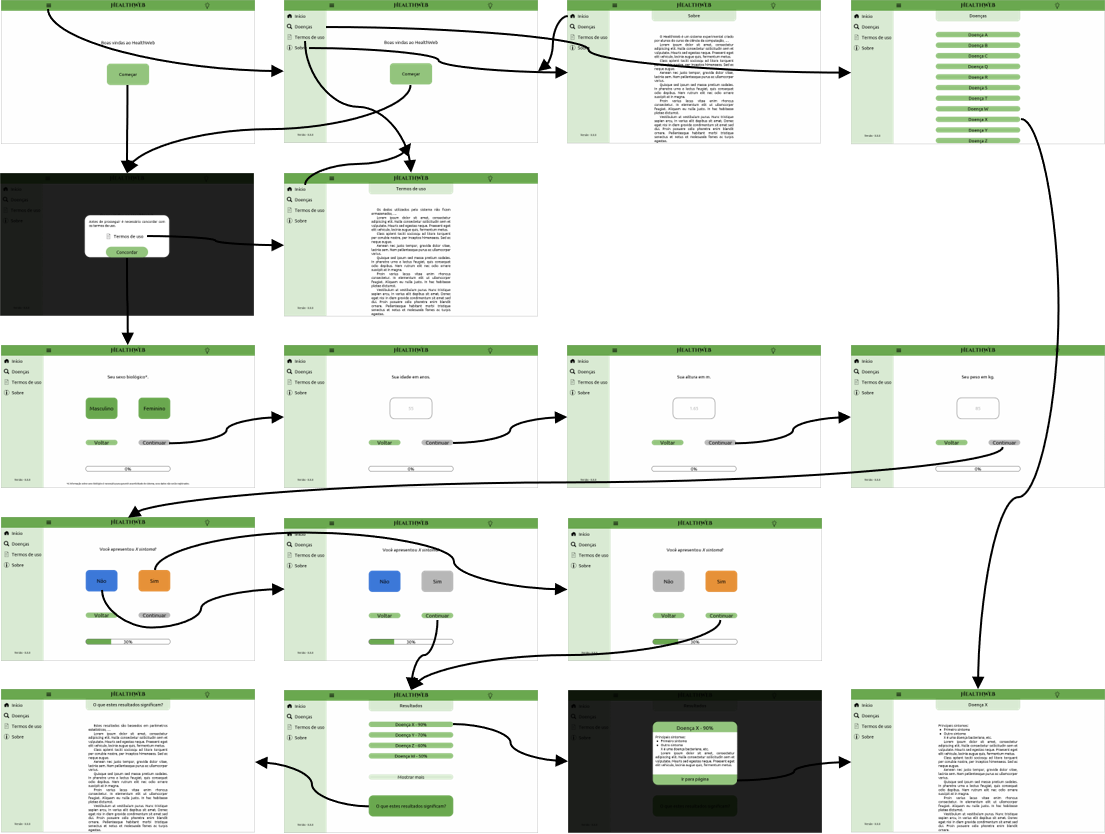
\includegraphics[width=\linewidth]{figure/prototype/desktop/storyboard.png}
	\caption{Storyboard para versão desktop.}
	\label{fig:desktop:story}
\end{figure}